\documentclass{iopconfser}
\usepackage{float}
\usepackage{graphicx}
\usepackage{subcaption}
\usepackage[automake]{glossaries-extra}
\usepackage{ragged2e}
\usepackage[export]{adjustbox}
\usepackage{mathtools}
\usepackage{setspace}
\onehalfspacing
% \makeglossaries

\setabbreviationstyle[acronym]{long-postshort-user}
\glssetcategoryattribute{acronym}{nohyperfirst}{true}
\setabbreviationstyle{short-nolong}
\makeglossaries

% --------------------
% ---- Glossaries ----
% --------------------
\newglossaryentry{asyncio}{name=Asyncio, description={A Python library for asynchronous code.}}
\newglossaryentry{stim}{name=STIM300, description={A MEMS-based \gls{imu}}}
\newglossaryentry{f9p}{name=F9P, description={A Global Navigation Satellite System (GNSS) receiver manufactured by u-blox.}}

% --------------------
% ----- Acronyms -----
% --------------------
\newacronym{asv}{ASV}{Autonomous Surface Vehicle}
\newacronym{dolp}{DoLP}{Degree of Linear Polarization}
\newacronym{aolp}{AoLP}{Angle of Linear Polarization}
\newacronym{sitaw}{SITAW}{Situational Awareness}
\newacronym{poe}{PoE}{Power over Ethernet}
\newacronym{pps}{PPS}{Pulse Per Second}
\newacronym{cpfa}{CPFA}{Color-Polarization Filter Array}
\newacronym{utc}{UTC}{Coordinated Universal Time}
\newacronym{imu}{IMU}{Inertial Measurement Unit}
\newacronym{tov}{TOV}{Time of Validity}
\newacronym{tm2}{TM2}{Time mark data}
\newacronym{gnss}{GNSS}{Global Navigation Satellite System}
\newacronym{ptp}{PTP}{Precision Time Protocol}

% \glsaddall
% \makenoidxglossaries

% \glsunset{cpu}
\glsunset{gnss}
\glsunset{imu}
\glsunset{tm2}
\glsunset{utc}

% --------------------
% ----- Shortcuts ----
% --------------------


\addbibresource{mylib.bib}
 

\begin{document}
\title{IØ8906 Submission}
% \author{Emil Martens}

\section*{Utilization Plan}
\subsection*{Problem / Solution}
I started my pitch by asking the audience to raise a hand if they depend in data to pertorm their research.
With 100\% of the audience raising their hand it is clear that data is a crucial part of research.
The type of data each researcher needs varies, of course, but in the field of robotics and autonomy almost every researcher needs to work with some sort of sensor data.
With this in mind, I have developped a sensor rig, depicted in Figure \ref{fig:operation}, to make it easier for researchers to perform data collection.
The sensor rig is designed for easy transport and operation by a single individual, and can also be temporarily attached to an existing vessel, making it versatile for a wide range of data collection scenarios.
As accurate positioning and synchronazation is key for any high quality dataset the sensor rig is equipped with two GNSS receivers and an IMU and everything is synchronized to UTC.
The sensor rig provides for separate gigabit ethernet ports with PoE to connect various sensors.
A custom web app is developed to control and monitor the sensor rig from a smartphone, making it easy to operate for almost anyone.
The fact that multiple different people have used the sensor sig with mimimal training is a testament to its usability.
At the end of the pitch I asked for funding hire a student over the summer to help developing the sensor rig further and use it collect data.
From holding a similar pitches in the past did get funding to hire not one but two students, signalling that the audience sees the potential in the sensor rig.


\begin{figure}[H]
    \centering
    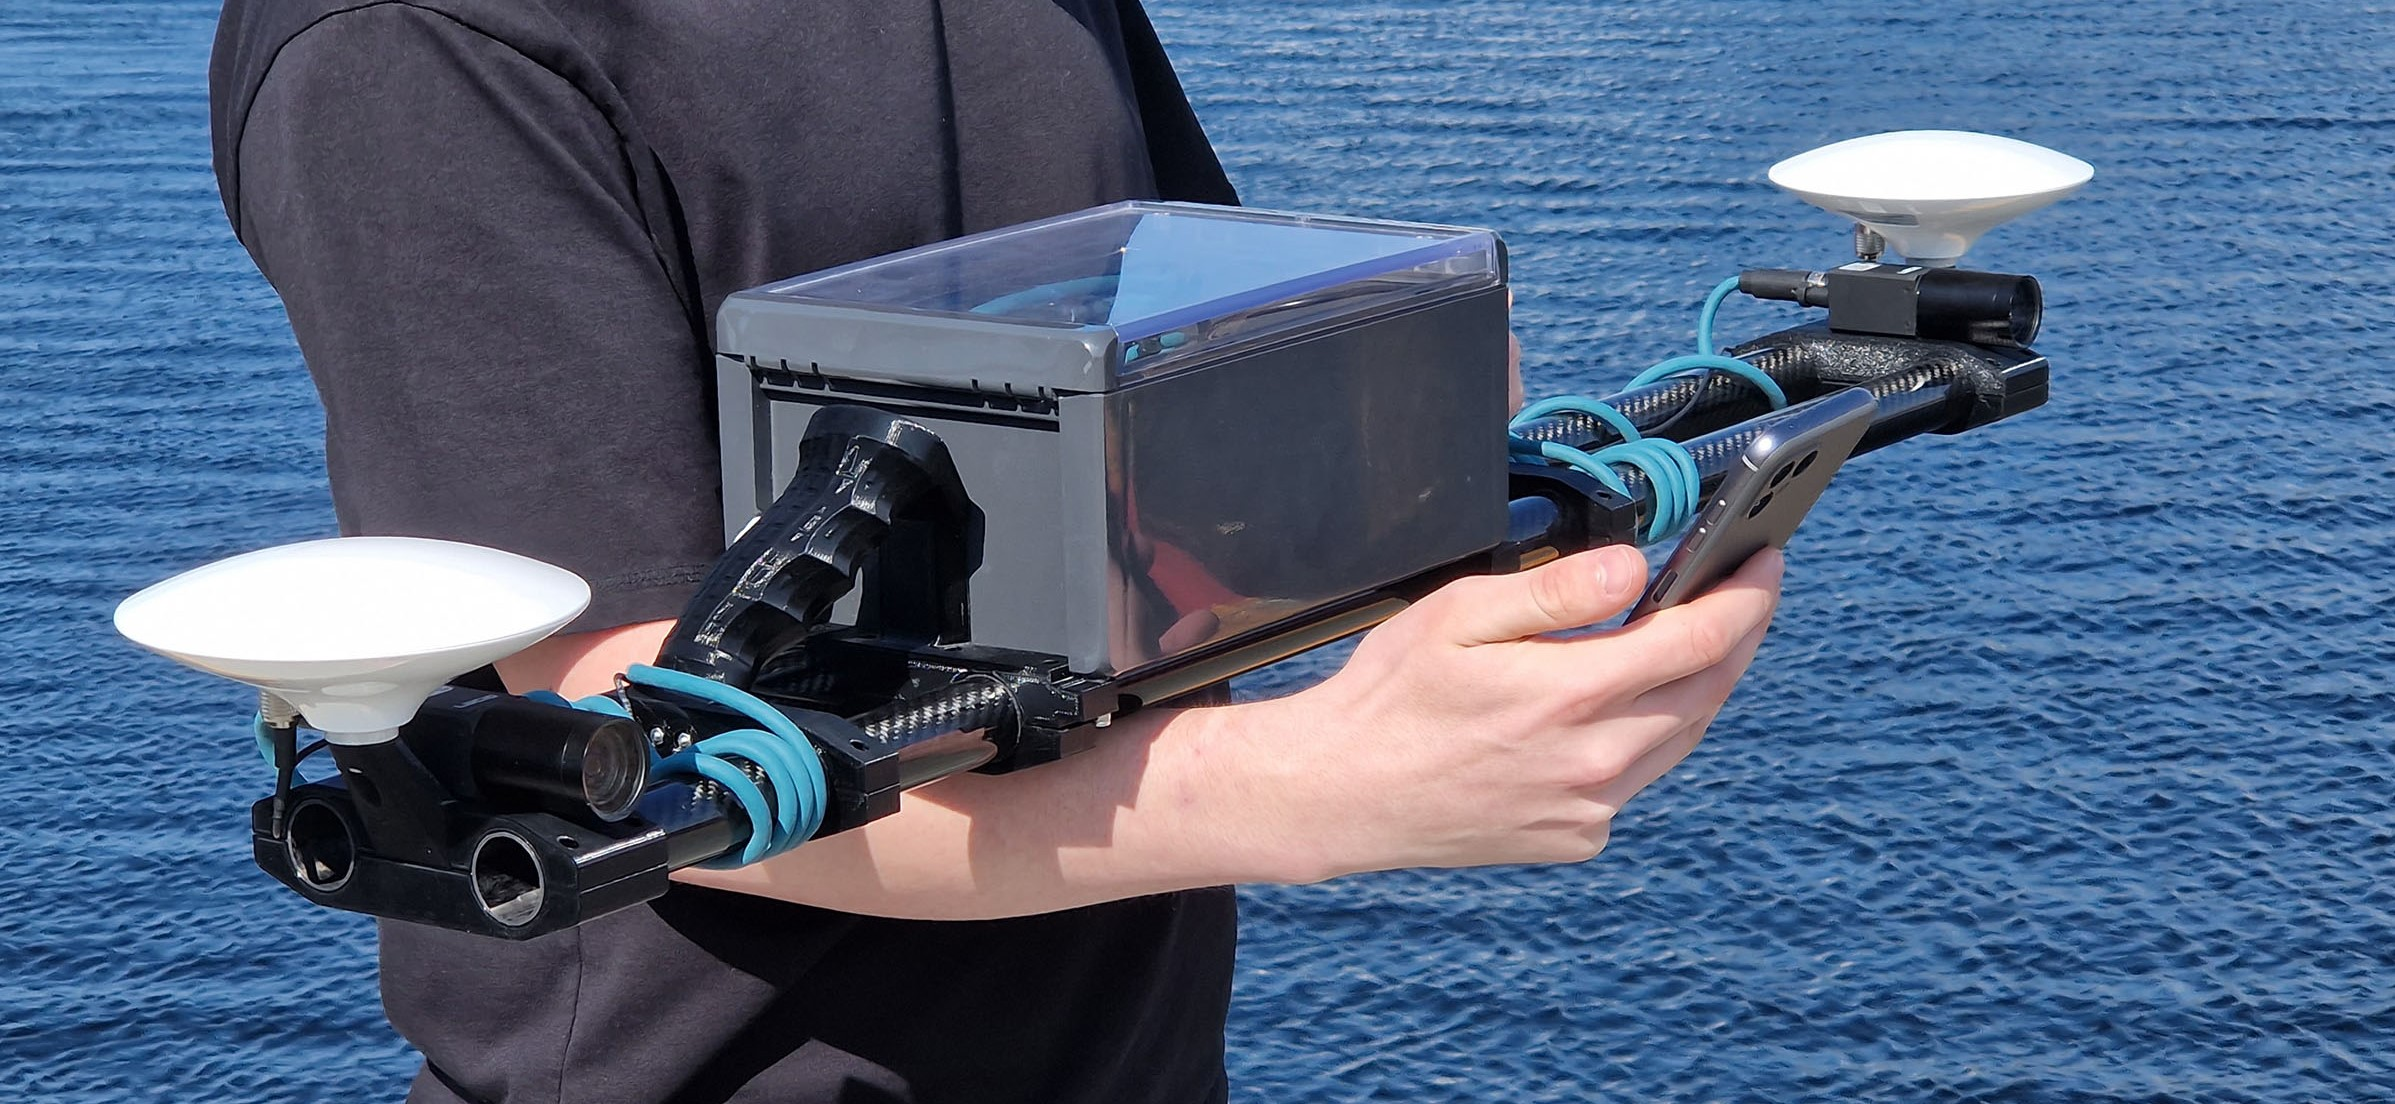
\includegraphics[trim={0 1cm 0 1cm},clip,width=\textwidth]{figures/operation.jpg}
    \caption{Human operation of the sensor rig with monitoring over a smartphone. \label{fig:operation}}
\end{figure}


\subsection*{Benefits}
From a users perspective, the key benefit of the sensor rig is its ease of use.
Research teams working in autonomy often rely on expensive research vehicles, such as the autonomous ferry Milliampere 2 to do their research.
These vehicles can be used to collect data, but it can be overkill and their operation often requires planning and coordination between multiple people.
If anything fails on the vehicle, even things not connected to data collection, such as a morot, the vehicle is generally taken out of operation

With the sensor rig, a single person can just pick it up, walk outside and start collecting data in a matter of minutes.
With its modular and stand alone desagn, it is also easy to attach it to an existing vehicle to temporarily create a pseudo research vehicle or expand the capabilities of an existing one.
Compared to any research vehicle, the sensor rig is also much cheaper, making it more accessible to smaller research teams.

\subsection*{Maret potential}
If the sensor rig was to be commercialized, it would be targeted towards small to medium sized research teams working in autonomy, as larger teams probably have dedicated hardware engineers to develop custom solutions.
A popential product would be the bare bone sensor rig equipped only with GNSS receivers an IMU and a the core computer.
Different brackets for attaching various sensors could be sold separately, as well as fully equipped versions with cameras and other sensors.
As the sensors used for researhing autonomy are generally expensive, having an easy way to use them as much as possible is valuable.
From personal experience I know researhers often have expensive sensors lying around that they do not use due to low usability.

The market potenteal for the sensor rig remains to be researched, but I believe there is a market for a product like this based on feedback from other researchers.

\subsection*{Existing competition}
I have not done a market analysis, but I am not aware of any similar product on the market.
One related prodct is the ZED-box from Stereolabs which can be used to collect data from multiple ZED cameras and synchronize them to UTC \cite{stereolabsZEDBoxEmbedded}. 
This is not a competitor to the sensor rig, but shows that there is a market for easy to use sensor synchronization systems.
Another related product is the SentiBoard from SentiSystems which handles synchronization of multiple sensors and can be used to calculate accurate position and orientation from GNSS and IMU data \cite{sentisystemsSentiSystemsSolutions}.
Both the ZED-box and the SentiBoard appear to be more aimed at the industrial market, and are not as versatile as the sensor rig.

\subsection*{Milestones}
The first milestone for the sensor rig was to develop a prototype and test it in a real research setting.
This milestone was reached in 2024, and the sensor rig has since been in use to collect data.
I submitted a paper describing the sensor rig to the ICMASS conference in 2024 and will present it there if accepted.
This is the next milestone will be a good opportunity to get feedback from the research community and to get the sensor rig known.

The following goal is to use the data from the sensor rig in my future publications and having other researchers use it in their research as well, proving the value of the sensor rig in a research setting.
Hopefully, when I finish my PhD in two years, the sensor rig will have a proven track record and be ready for commercialization.

If I decide to pursue commercialization, the next milestone would be to sell a couple units to other research teams and provide good customer support to get feedback on the product.
This should not require much investment nor time and can be done as a side job if I reduce my main job to part time.

The end goal wouid be to sell the sensor rig as a finished product with a thurough user guide and have it be used by research teams all over the world with minimal support.


\subsection*{Commercialization}
A key advantage with the commercialization of the sensor rig is that it requires very little investment to get started. 
The rig is an assembly of off-the-shelf components and 3D printed parts coupled with software that has already been developed.


\section*{Reflection note}

\section*{Intelectual Property}
\section*{References}
% \printbibliography

\end{document}